One of Dr. Jonas' greatest discoveries was the democratic nation
of Heyting people, who kept meticulous records of their elections 
and their rulers.
Strangely, even though the Heyting people were democratic, 
their voting records indicated that many of their elected officials
recived far less than the majority of the votes.
How could this happen?

Well, to simplify the voting process, each of the Heyting tribes had broken their 
land up into districts.
Each district had one vote for the next ruler of that tribe, which was based upon
the majority vote from within the district.
However, since the existing tribe leaders were allowed to draw the boundaries 
of the districts as long as they respected the following guidelines,
the minority party X was able to keep power from the majority party O.
\begin{enumerate}
\item Each district had to be a single connected region.
\item Each district needed to contain a single temple (marked as stars on the maps).
\item The difference in population between any two districts had to be 5 or less.
\item All district boundary lines had to follow the horizontal and vertical grid lines provided.
\end{enumerate}

For each of the four tribes, find a way to draw the district lines such that party X
has strictly more votes than party O in more than half of the total districts.
Then enter the total population (Xs and Os) for each of the capital districts (containing
the biggest star) into
ClueKeeper using the following format: \texttt{A\#\#-B\#\#-C\#\#-D\#\#}.

I'm attaching an example Tribe Z. Note that its solution would be entered into ClueKeeper as \texttt{Z19}
since the captial district has 19 people. -BF

\hfill
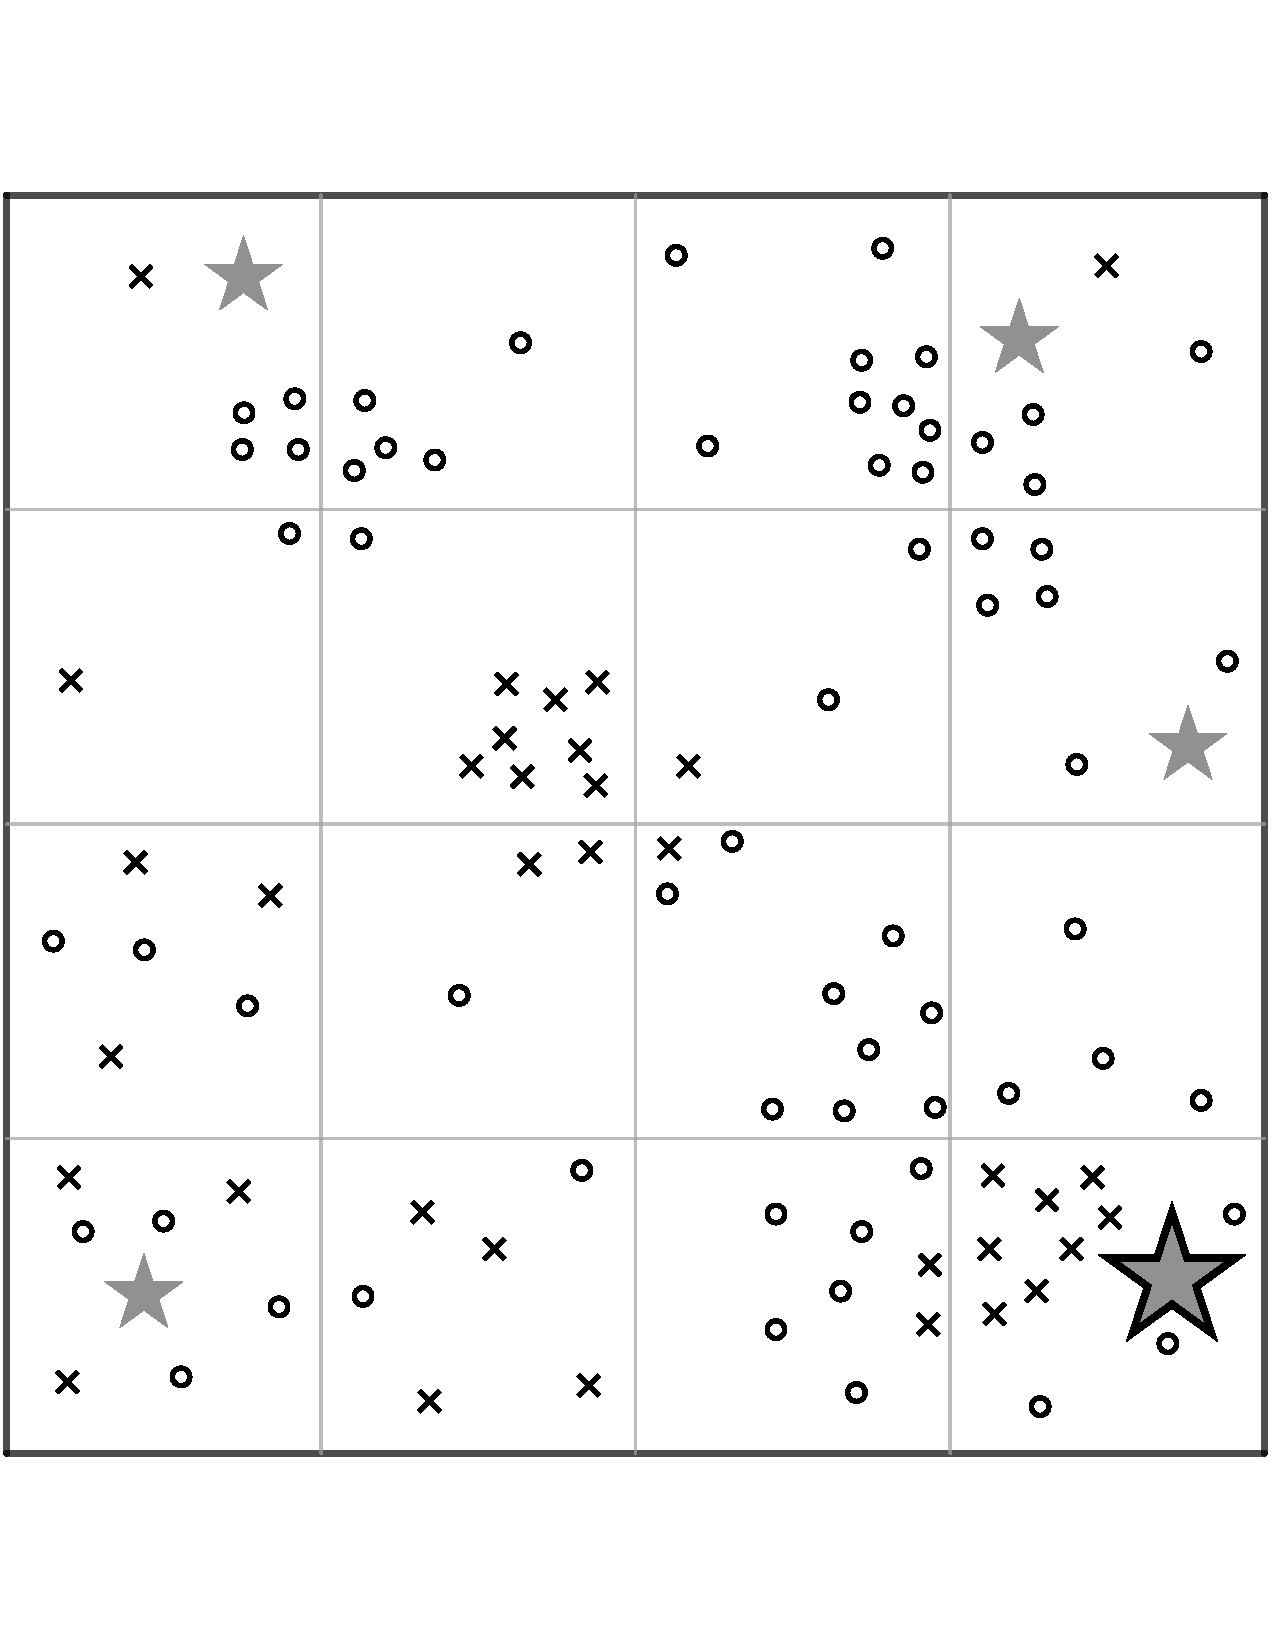
\includegraphics[width=2.5in]{assets/gerrymander-example.pdf} 
\hfill
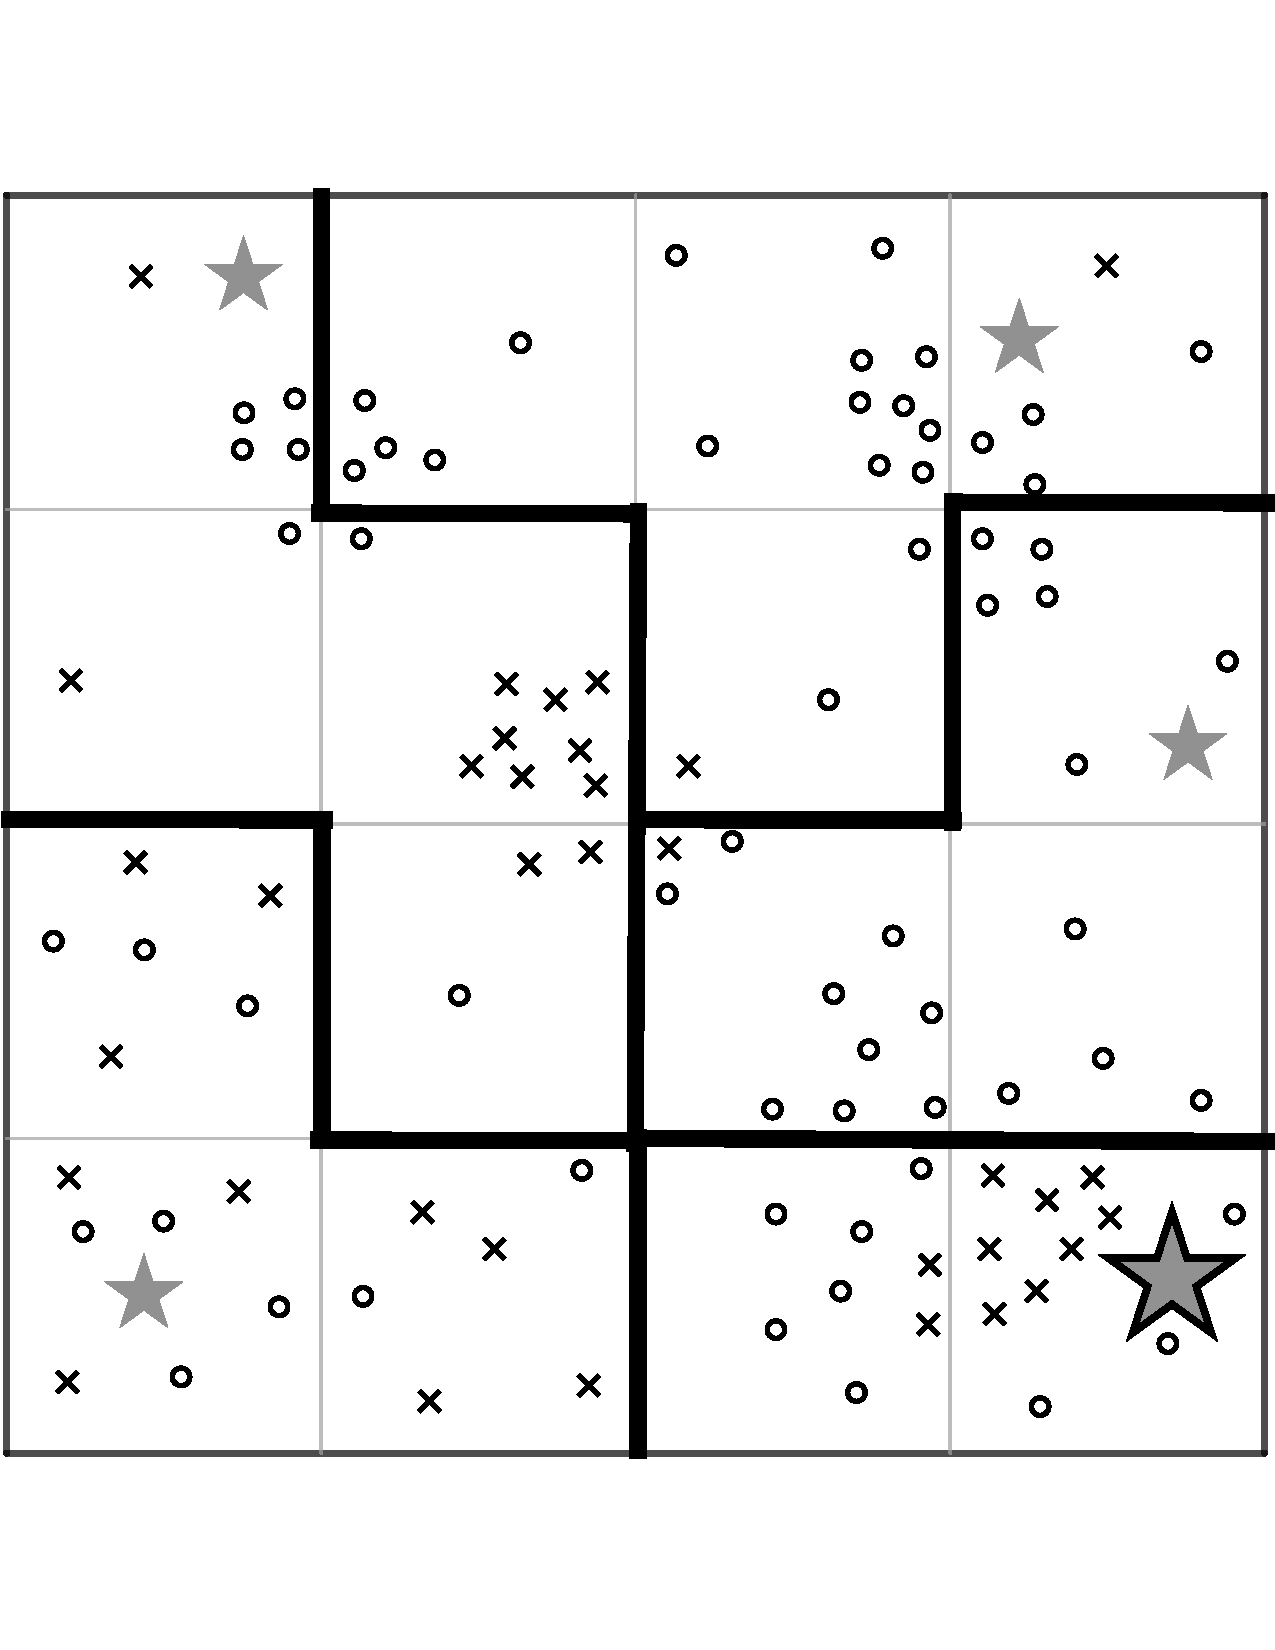
\includegraphics[width=2.5in]{assets/gerrymander-example-solution.pdf}
\hfill\phantom{}
